\documentclass[10pt,a4paper]{article}
\usepackage{amssymb} %mathbb
\usepackage{amsmath} %align
\usepackage{eucal}
\usepackage{hyperref}
\usepackage{cancel}
\usepackage{array,bm}
\usepackage{graphicx} %jpg
\usepackage{tikz-cd}
\usetikzlibrary{arrows, matrix}
\usepackage[top=1.0cm,bottom=1.3cm,left=1.0cm,right=1.0cm]{geometry}
\newcolumntype{C}{>{$}c<{$}}
\renewcommand{\arraystretch}{1.2}
\begin{document}
	\Large

	\begin{center}
		Lista de Geometria de Riemann, Vin\'icius Claudino Ferraz
	\end{center}

	\normalsize

Tensorial Video on \href{https://www.youtube.com/watch?v=mmzqmIcX7xo}{\color{blue}\underline{YouTube}}. Riemannian Geometry Video on \href{https://www.youtube.com/watch?v=Z3IXeWvEEa4}{\color{blue}\underline{YouTube}}.

	\section{$F: \mathbb{C} \rightarrow \mathbb{C} \,; F(w) = z$}
		\begin{flushright}
		\end{flushright}

		$w = u + vi = \rho e^{i\theta}, z = x + yi = r e^{it}$. Provar que $F^* (\mathrm{d}z \, \mathrm{d}\overline{z}) = \vert F'(w) \, \vert^2\, \mathrm{d}w \, \mathrm{d}\overline{w}$.

		$(\mathrm{d}x + i \mathrm{d}y) \wedge (\mathrm{d}x - i \mathrm{d}y) = - 2i \, \mathrm{d}x \wedge \mathrm{d}y \Rightarrow (\mathrm{d}u + i \mathrm{d}v) \wedge (\mathrm{d}u - i \mathrm{d}v) = - 2i \, \mathrm{d}u \wedge \mathrm{d}v$

		$F^* (- 2i \,\mathrm{d}x \wedge \mathrm{d}y) = -2i \, F^* (\mathrm{d}x \wedge \mathrm{d}y) = -2i\, F^* (\mathrm{d}x) \wedge F^*(\mathrm{d}y) = -2i (x_u \mathrm{d}u + x_v \mathrm{d}v) \wedge (y_u \mathrm{d}u + y_v \mathrm{d}v)$

		$= -2i (x_u y_v \mathrm{d}u \wedge \mathrm{d}v + x_v y_u \mathrm{d}v \wedge \mathrm{d}u) = -2i (\det J) \mathrm{d}u \wedge \mathrm{d}v \Rightarrow \vert F'(w) \vert^2 = \det J \Rightarrow F'(w) = f + gi$

		$\cfrac{\partial z}{\partial u} = \cfrac{\mathrm{d}z}{\mathrm{d}w} \, \cdot \cancel{\cfrac{\partial w}{\partial u}} \Rightarrow \cfrac{\mathrm{d}z}{\mathrm{d}w} = \cfrac{\partial z}{\partial u} = -i \cdot \cfrac{\partial z}{\partial v} = e^{-i\theta} \cfrac{\partial z}{\partial \rho} = -\cfrac{i}{\rho e^{i\theta}} \cdot \cfrac{\partial z}{\partial \theta}$

		$\therefore \cfrac{\mathrm{d}F}{\mathrm{d}w} = \cfrac{\partial F}{\partial u} = -i \cdot \cfrac{\partial F}{\partial v} = e^{-i\theta} \cfrac{\partial F}{\partial \rho} = -\cfrac{i}{\rho e^{i\theta}} \cdot \cfrac{\partial F}{\partial \theta}$

		\vspace{3mm}

		$x = r \cos t, y = r \sin t, u = \rho \cos \theta, v = \rho \sin \theta$

		d$z = \mathrm{d}F_{(u,v)} = \left[ \begin{matrix} \cfrac{\partial x}{\partial u} & \cfrac{\partial x}{\partial v} \\ \cfrac{\partial y}{\partial u} & \cfrac{\partial y}{\partial v} \end{matrix} \right] = \left[ \begin{matrix} f & -g \\ g & f \end{matrix} \right] = \left[ \begin{matrix} x_r r_u + x_t t_u & x_r r_v + x_t t_v \\ y_r r_u + y_t t_u & y_r r_v + y_t t_v \end{matrix} \right] = \left[ \begin{matrix} r_u \cos t - t_u r \sin t & r_v \cos t - t_v r \sin t \\ r_u \cos t + t_u r \cos t & r_v \cos t + t_v r \cos t \end{matrix} \right]$

		$f = r_u \cos t - t_u r \sin t = r_v \cos t + t_v r \cos t \Rightarrow [r_u - r_v - t_v r] \cos t = t_u r \sin t$

		$g = r_u \cos t + t_u r \cos t = - r_v \cos t + t_v r \sin t \Rightarrow [r_u + t_u r + r_v] \cos t = t_v r \sin t$

		Temos $r_u, r_v, t_u, t_v, r, \tan t$ e podemos eliminar 2 em fun\c{c}\~ao do resto.

		$r \tan t = \cfrac{r_u - r_v - t_v r}{t_u} = \cfrac{r_u + t_u r + r_v}{t_v} \Rightarrow r = \cfrac{r_u - r_v}{t_v + t_u \tan t} = \cfrac{r_u + r_v}{t_v \tan t - t_u} = \cfrac{1}{A} r_u - \cfrac{1}{A} r_v = \cfrac{1}{B} r_u + \cfrac{1}{B} r_v $

		$r_v = r_u \cfrac{B - A}{B + A} \Rightarrow r_u - r_u \cfrac{B - A}{B + A} = Ar \Rightarrow r_u = r \cfrac{B + A}{2} \Rightarrow r_v =  r \cfrac{B - A}{2}$

		$\therefore \cfrac{r_u}{r} = \cfrac{t_v \tan t - t_u + t_v + t_u \tan t}{2} \Rightarrow \cfrac{r_v}{r} =  \cfrac{t_v \tan t - t_u - t_v - t_u \tan t}{2}$ Separei as vari\'aveis.

		$\therefore \cfrac{\partial^2}{\partial u \partial v} (2 \ln r + t) = \cfrac{\partial}{\partial v} [t_v \tan t + t_v + t_u \tan t] = \cfrac{\partial}{\partial u} [t_v \tan t - t_u - t_u \tan t]$

		$\sin t \cos t (t_{uu} - 2t_{uv} + t_{vv}) + t_{uu} + t_{vv} + (t_u - t_v)^2 = 0$

		$\therefore \left( \begin{matrix} 1 \\ 1 \end{matrix} \right) r_u \cos t + \left( \begin{matrix} -1 \\ + 1 \end{matrix} \right) r_v \cos t + \left( \begin{matrix} - \sin t \\ \cos t \end{matrix} \right) t_u r + \left( \begin{matrix} - \cos t \\ - \sin t \end{matrix} \right) t_v r = 0$

		d$z = \mathrm{d}(r,t)_{(u,v)} = \left[ \begin{matrix} \cfrac{\partial r}{\partial u} & \cfrac{\partial r}{\partial v} \\ \cfrac{\partial t}{\partial u} & \cfrac{\partial t}{\partial v} \end{matrix} \right] = \left[ \begin{matrix} r_x x_u + r_y y_u & r_x x_v + r_y y_v \\ t_x x_u + t_y y_u & t_x x_v + t_y y_v  \end{matrix} \right] = \left[ \begin{matrix} f \cfrac{x}{\sqrt{x^2+y^2}} + g \cfrac{y}{\sqrt{x^2+y^2}} & - g \cfrac{x}{\sqrt{x^2+y^2}} + f \cfrac{y}{\sqrt{x^2+y^2}} \\ - f \cfrac{y}{x^2+y^2} + g \cfrac{x}{x^2+y^2} & g \cfrac{y}{x^2+y^2} + f \cfrac{x}{x^2+y^2}  \end{matrix} \right]$

		d$z = \mathrm{d}(r,t)_{(\rho,\theta)} = \left[ \begin{matrix} \cfrac{\partial r}{\partial \rho} & \cfrac{\partial r}{\partial \theta} \\ \cfrac{\partial t}{\partial \rho} & \cfrac{\partial t}{\partial \theta} \end{matrix} \right] = \left[ \begin{matrix} r_x x_\rho + r_y y_\rho & r_x x_\theta + r_y y_\theta \\ t_x x_\rho + t_y y_\rho & t_x x_\theta + t_y y_\theta \end{matrix} \right] = \left[ \begin{matrix} x_\rho\cfrac{x}{\sqrt{x^2+y^2}} + y_\rho\cfrac{y}{\sqrt{x^2+y^2}} & x_\theta\cfrac{x}{\sqrt{x^2+y^2}} + y_\theta\cfrac{y}{\sqrt{x^2+y^2}} \\ - x_\rho \cfrac{y}{x^2+y^2} + y_\rho\cfrac{x}{x^2+y^2} & - x_\theta\cfrac{y}{x^2+y^2} + y_\theta\cfrac{x}{x^2+y^2} \end{matrix} \right]$

		d$z = \mathrm{d}(x,y)_{(\rho,\theta)} = \left[ \begin{matrix} \cfrac{\partial x}{\partial \rho} & \cfrac{\partial x}{\partial \theta} \\ \cfrac{\partial y}{\partial \rho} & \cfrac{\partial y}{\partial \theta} \end{matrix} \right] = \left[ \begin{matrix} x_u u_\rho + x_v v_\rho & x_u u_\theta + x_v v_\theta \\ y_u u_\rho + y_v v_\rho & y_u u_\theta + y_v v_\theta \end{matrix} \right] = \left[ \begin{matrix} f \cos \theta -g \sin \theta & - f \rho \sin \theta -g \rho \cos \theta \\ g \cos \theta + f \sin \theta & - g  \rho \sin \theta + f  \rho \cos \theta \end{matrix} \right]$

		d$z = \mathrm{d}(x,y)_{(r,t)} = \left[ \begin{matrix} \cos t & - r \sin t \\ \sin t & r \cos t \end{matrix} \right] = \left[ \begin{matrix} \cfrac{x}{\sqrt{x^2+y^2}} & - y \\ \cfrac{y}{\sqrt{x^2+y^2}} & x \end{matrix} \right]$

		d$w = \mathrm{d}(u,v)_{(\rho,\theta)} = \left[ \begin{matrix} \cos \theta & - \rho \sin \theta \\ \sin \theta & \rho \cos \theta \end{matrix} \right] = \left[ \begin{matrix} \cfrac{u}{\sqrt{u^2+v^2}} & - v \\ \cfrac{v}{\sqrt{u^2+v^2}} & u \end{matrix} \right]$

		$x > 0, t \in (-90^\circ, 90^\circ) \Rightarrow \mathrm{d}z = \mathrm{d}(r,t)_{(x,y)} = \left[ \begin{matrix} \cfrac{x}{\sqrt{x^2 + y^2}} & \cfrac{y}{\sqrt{x^2 + y^2}} \\ -\cfrac{y}{x^2 + y^2} & \cfrac{x}{x^2 + y^2} \end{matrix} \right] = \left[ \begin{matrix} \cos t & \sin t \\ - \cfrac{1}{r} \sin t & \cfrac{1}{r} \cos t \end{matrix} \right]$

		$u > 0, \theta \in (-90^\circ, 90^\circ) \Rightarrow \mathrm{d}w = \mathrm{d}(\rho,\theta)_{(u,v)} = \left[ \begin{matrix} \cfrac{u}{\sqrt{u^2 + v^2}} & \cfrac{v}{\sqrt{u^2 + v^2}} \\ -\cfrac{v}{u^2 + v^2} & \cfrac{u}{u^2 + v^2} \end{matrix} \right]  = \left[ \begin{matrix} \cos \theta & \sin \theta \\ - \cfrac{1}{\rho} \sin \theta & \cfrac{1}{\rho} \cos \theta \end{matrix} \right]$

		\section{C\'alculo 2 $-$ Matriz jacobiana da inversa}
		\begin{flushright}
		\end{flushright}

		Sejam $G = F^{-1}, F(u,v) = (x, y) = (x(u,v), y(u,v)) \Rightarrow dF_{(u,v)} = \left( \begin{matrix} x_u(u,v) & x_v(u,v) \\ y_u(u,v) & y_v(u,v) \end{matrix} \right)$

		$G(x,y) = (u,v) = (u(x,y), v(x,y)) = (u(x(u,v), y(u,v)), v(x(u,v), y(u,v))) \Rightarrow dG_{(x,y)} = \left( \begin{matrix} u_x(x,y) & u_y(x,y) \\ v_x(x,y) & v_y(x,y) \end{matrix} \right)$

		$I(u,v) = (u,v) \Rightarrow G \circ F = I \Rightarrow u = u(x(u,v),y(u,v)), v = v(x(u,v),y(u,v))$

		Pela regra da cadeia, $dI_{(u,v)} = dG_{(x,y)} \cdot dF_{(u,v)}$.

		\begin{align*}
		x_u u_x + x_v v_x &= 1 \\
		x_u u_y + x_v v_y &= 0 \\
		y_u u_x + y_v v_x &= 0 \\
		y_u u_y + y_v v_y &= 1
		\end{align*}

		$\therefore u_x = \cfrac{\det \left( \begin{matrix} 1 & x_v(u,v) \\ 0 & y_v(u,v) \end{matrix} \right)}{\det dF}\,;v_x = \cfrac{\det \left( \begin{matrix} x_u(u,v) & 1 \\ y_u(u,v) & 0 \end{matrix} \right)}{\det dF},\;u_y = \cfrac{\det \left( \begin{matrix} 0 & x_v(u,v) \\ 1 & y_v(u,v) \end{matrix} \right)}{\det dF}\,;v_y = \cfrac{\det \left( \begin{matrix} x_u(u,v) & 0 \\ y_u(u,v) & 1 \end{matrix} \right)}{\det dF}\,\,\blacksquare$

		Em geral, existe uma f\'ormula para as entradas da matriz jacobiana inversa, calculado em um ponto do dom\'inio de $F$.

	\section{$F^* (T^n \otimes U^n) = F^* T^n \otimes F^* U^n$}
		\begin{flushright}
		\end{flushright}

		Seja $F: M \rightarrow N$ aplica\c{c}\~ao diferenci\'avel entre variedades diferenci\'aveis.  $T^m \in \mathcal{T}^k(M), T^n \in \mathcal{T}^k(N)$.

		$p \in M, F(p) = q \in N, w_i = dF_p (v_i)$. Ent\~ao: $F^* T^n = T^m$ se $T^m_p (v_1, \cdots, v_k) = T_q^n (w_1, \cdots, w_k)$.

		\vspace{3mm}

		Expressamos $T_p^m$ na base de $du^1 \otimes \cdots \otimes du^k$, com todos os \'indices variando de $1$ a $\Delta_m$. Chamamos as coordenadas de $\alpha_i^m$, com $i$ variando de $1$ a $\Delta_m^k$.

		\vspace{3mm}

		Expressamos $U_p^m$ na base de $du^1 \otimes \cdots \otimes du^k$, com todos os \'indices variando de $1$ a $\Delta_m$. Chamamos as coordenadas de $\beta_i^m$, com $i$ variando de $1$ a $\Delta_m^k$.

		\vspace{3mm}

		Logo, $V_p^m = T_p^m \otimes U_p^m = \sum \alpha_i^m \beta_j^m (du^1 \otimes \cdots \otimes du^k) \otimes (du^1 \otimes \cdots \otimes du^k) \in \mathcal{T}^{2k}(M)$.

		\vspace{3mm}

		Expressamos $T_q^n$ na base de $dx^1 \otimes \cdots \otimes dx^k$, com todos os \'indices variando de $1$ a $\Delta_n$. Chamamos as coordenadas de $A_i$, com $i$ variando de $1$ a $\Delta_n^k$.

		\vspace{3mm}

		Expressamos $U_q^n$ na base de $dx^1 \otimes \cdots \otimes dx^k$, com todos os \'indices variando de $1$ a $\Delta_n$. Chamamos as coordenadas de $B_i$, com $i$ variando de $1$ a $\Delta_n^k$.

		\vspace{3mm}

		Logo, $V_q^n = T_q^n \otimes U_q^n = \sum A_i B_j (dx^1 \otimes \cdots \otimes dx^k) \otimes (dx^1 \otimes \cdots \otimes dx^k) \in \mathcal{T}^{2k}(N)$.

		\vspace{3mm}

		Queremos mostrar que $F_* V_p^m = V_q^n$.

		Por defini\c{c}\~ao $V^m_p (v_1, \cdots, v_{2k}) = V_q^n (w_1, \cdots, w_{2k})$.

		\vspace{3mm}

		Substituindo $w_i = dF_p(v_i) \Rightarrow \alpha_i^m = \text{Tran}_i^1(A_1, \cdots, A_j)$, com $j = \Delta_n^k$ e com $i$ variando de $1$ a $\Delta_m^k$.

		\vspace{3mm}

		Tamb\'em, $\beta_i^m = \text{Tran}_i^1(B_1, \cdots, B_j)$, com $j = \Delta_n^k$ e com $i$ variando de $1$ a $\Delta_m^k$.

		\vspace{3mm}

		Tamb\'em, $\gamma_K^m = \text{Tran}_K^2(C_1, \cdots, C_L)$, com $L = 2\Delta_n^{2k}$ e com $K$ variando de $1$ a $2\Delta_m^{2k}$.

		$\gamma_K^m = \alpha_i^m \beta_j^m$

		$C_L = A_i B_j$

		$\alpha_i^m \beta_j^m = \text{Tran}_i^1(A_1, \cdots, A_L) \text{Tran}_j^1(B_1, \cdots, B_L) = \text{Tran}_{ij}^2(A_1 B_1, \cdots, A_L B_L)$, com $L= \Delta_n^k$.

		\vspace{3mm}

		Baixando o n\'ivel,

		$\alpha_1^m = A_1^1 \xi_u^2  + A_2^1 \xi_u \sigma_u  + A_3^1 \xi_u \tau_u$
		$+ A_1^2 \sigma_u \xi_u  + A_2^2 \sigma_u^2  + A_3^2 \sigma_u \tau_u$
		$+ A_1^3 \tau_u \xi_u  + A_2^3 \tau_u \sigma_u  + A_3^3 \tau_u^2 = \text{Tran}_1^1(A_1,A_2,A_3)$

		$\beta_1^m = B_1^1 \xi_u^2  + B_2^1 \xi_u \sigma_u  + B_3^1 \xi_u \tau_u$
		$+ B_1^2 \sigma_u \xi_u  + B_2^2 \sigma_u^2  + B_3^2 \sigma_u \tau_u$
		$+ B_1^3 \tau_u \xi_u  + B_2^3 \tau_u \sigma_u  + B_3^3 \tau_u^2 = \text{Tran}_1^1(B_1,B_2,B_3)$

		Multiplique ambos. Conseguir\'a um polin\^omio de grau sempre $4 = 2k$. $9 \times 9 = 3^{2k}$ mon\^omios.

		Existe uma \'unica forma linear de combinar mon\^omios de grau $k$ e gerar mon\^omios de grau $2k$: multiplicando os coeficientes.

		O teorema segue por linearidade e pelo fato de todos os mon\^omios do sistema principal serem de grau $k.\,\,\blacksquare$

		\subsection{Tensores covariantes, Bases contravariantes}
		\begin{flushright}
		\end{flushright}

		Vamos subir para $V^m \in \mathcal{T}_2^0(M)$

		$V^m : M \rightarrow T_2^0 M$

		$p \mapsto (p, T'), T' \in T_2^0(T_pM)$

		$T' : T_p^*M \times T_p^*M \rightarrow \mathbb{R}$

		$(\omega_1, \omega_2) \mapsto V_p^m(\omega_1, \omega_2)$. Lembrando que os covetores tangentes satisfazem $\omega_p : C^\infty(M) \rightarrow \mathbb{R} \,; f \mapsto \omega_p(f) $.

		Em $\mathcal{T}_1^0(M), \,\,T'(\omega_1) = (\alpha \partial_u + \beta \partial_v) (\omega_1)$.

		(Aqui eu deveria ter simplificado: $\omega_1 = \omega_2 = \omega, \eta_1 = \eta_2 = \eta$).

		$V_p^m(\omega_1, \omega_2) = \alpha^m \partial_u \otimes \partial_u (\omega_1, \omega_2) + \beta^m \partial_u \otimes \partial_v (\omega_1, \omega_2) + \gamma^m \partial_v \otimes \partial_u (\omega_1, \omega_2) + \delta^m \partial_v \otimes \partial_v (\omega_1, \omega_2)$

		Vamos precisar da dimens\~ao do espa\c{c}o em que $M$ est\'a imerso. Sejam $\dim M + \text{codim } M = \Delta_m, \dim N + \text{codim } N = \Delta_n$.

		Em geral, expressamos $T_p^m$ na base de $\partial_u^1 \otimes \cdots \otimes \partial_u^k$, com todos os \'indices variando de $1$ a $\Delta_m$. Chamamos as coordenadas de $\alpha_i^m$, com $i$ variando de $1$ a $\Delta_m^k$.

		\vspace{3mm}

		$V_p^m(\omega_1, \omega_2) = \alpha^m \omega_1^1 \omega_2^1 + \beta^m \omega_1^1 \omega_2^2 + \gamma^m \omega_1^2 \omega_2^1 + \delta^m \omega_1^2 \omega_2^2$

		$W_q^n(\eta_1, \eta_2) = V_p^m(\omega_1, \omega_2)$ com $F^*\eta_i = \omega_i = (J\pi^{-1}_p)^T \cdot \eta_i \Rightarrow \omega_i^1 = \xi_u \eta_i^1 + \sigma_u \eta_i^2 + \tau_u \eta_i^3 \Rightarrow \omega_i^2 = \xi_v \eta_i^1 + \sigma_v \eta_i^2 + \tau_v \eta_i^3$

		\textbf{LINHA 1:} Em geral, $T_q^n(\eta_1,\cdots,\eta_k) = T_p^m(\omega_1, \cdots, \omega_k)$. Transposta da matriz jacobiana de $F$.

		\vspace{3mm}

		$W_q^n(\eta_1, \eta_2) = A^1 \partial_\xi \otimes \partial_\xi + A^2 \partial_\xi \otimes \partial_\sigma + A^3 \partial_\xi \otimes \partial_\tau $
		$+ A^4 \partial_\sigma \otimes \partial_\xi + A^5 \partial_\sigma \otimes \partial_\sigma + A^6 \partial_\sigma \otimes \partial_\tau $
		$+ A^7 \partial_\tau \otimes \partial_\xi + A^8 \partial_\tau \otimes \partial_\sigma + A^9 \partial_\tau \otimes \partial_\tau $

		Em geral, expressamos $T_q^n$ na base de $\partial_{x^1} \otimes \cdots \otimes \partial_{x^k}$, com todos os \'indices variando de $1$ a $\Delta_n$. Chamamos as coordenadas de $A_i$, com $i$ variando de $1$ a $\Delta_n^k$.

		\vspace{3mm}

		$V_p^m(\omega_1, \omega_2) = \alpha^m (\xi_u \eta_1^1 + \sigma_u \eta_1^2 + \tau_u \eta_1^3) (\xi_u \eta_2^1 + \sigma_u \eta_2^2 + \tau_u \eta_2^3) + \beta^m (\xi_u \eta_1^1 + \sigma_u \eta_1^2 + \tau_u \eta_1^3) (\xi_v \eta_2^1 + \sigma_v \eta_2^2 + \tau_v \eta_2^3)$

		$+ \gamma^m (\xi_v \eta_1^1 + \sigma_v \eta_1^2 + \tau_v \eta_1^3) (\xi_u \eta_2^1 + \sigma_u \eta_2^2 + \tau_u \eta_2^3) + \delta^m (\xi_v \eta_1^1 + \sigma_v \eta_1^2 + \tau_v \eta_1^3) (\xi_v \eta_2^1 + \sigma_v \eta_2^2 + \tau_v \eta_2^3)$

		\vspace{3mm}

		Em geral, tamb\'em \'e poss\'ivel trocar todos os $\omega_i$ pelas transpostas das matrizes jacobianas de $F$ vezes $\eta_i$.

		\vspace{3mm}

		$V_p^m(\omega_1, \omega_2) = \alpha^m (\xi_u \partial_\xi + \sigma_u \partial_\sigma + \tau_u \partial_\tau) \otimes (\xi_u \partial_\xi + \sigma_u \partial_\sigma + \tau_u \partial_\tau) + \beta^m (\xi_u \partial_\xi + \sigma_u \partial_\sigma + \tau_u \partial_\tau) \otimes (\xi_v \partial_\xi + \sigma_v \partial_\sigma + \tau_v \partial_\tau)$

		$+ \gamma^m (\xi_v \partial_\xi + \sigma_v \partial_\sigma + \tau_v \partial_\tau) \otimes (\xi_u \partial_\xi + \sigma_u \partial_\sigma + \tau_u \partial_\tau) + \delta^m (\xi_v \partial_\xi + \sigma_v \partial_\sigma + \tau_v \partial_\tau) \otimes (\xi_v \partial_\xi + \sigma_v \partial_\sigma + \tau_v \partial_\tau)$

		\vspace{3mm}

		$V_p^m = B^1 \partial_\xi \otimes \partial_\xi + B^2 \partial_\xi \otimes \partial_\sigma + B^3 \partial_\xi \otimes \partial_\tau $
		$+ B^4 \partial_\sigma \otimes \partial_\xi + B^5 \partial_\sigma \otimes \partial_\sigma + B^6 \partial_\sigma \otimes \partial_\tau $
		$+ B^7 \partial_\tau \otimes \partial_\xi + B^8 \partial_\tau \otimes \partial_\sigma + B^9 \partial_\tau \otimes \partial_\tau $

		\vspace{3mm}

		O sistema \textbf{PRINCIPAL} \'e:

		$A^i = B^i(\alpha^m, \beta^m, \gamma^m, \delta^m)$, com $i$ variando de $1$ a $9$.

		\vspace{3mm}

		Em geral, $A^i = B^i(\alpha_1^m, \cdots, \alpha_j^m)$, com $j = \Delta_m^k$ e com $i$ variando de $1$ a $\Delta_n^k$.

		\vspace{3mm}

		\textbf{LINHA 2:} Multiplique por $g$: $X_p^m(\omega_1, \omega_2) = g V_p^m(\omega_1, \omega_2)$.

		Em geral, $U_p^m(\omega_1, \cdots, \omega_k) = g T_p^m(\omega_1, \cdots, \omega_k)$.

		\vspace{3mm}

		Calcular o push forward de $X_p^m = \left( \begin{matrix} f(\xi, \sigma, \tau) \alpha^m \\ f(\xi, \sigma, \tau) \beta^m \\ f(\xi, \sigma, \tau) \gamma^m \\ f(\xi, \sigma, \tau) \delta^m \end{matrix} \right)$ e encontrar $Y_q^n = \left( \begin{matrix} f(\xi, \sigma, \tau) A^1 \\ \vdots \\  f(\xi, \sigma, \tau) A^9 \end{matrix} \right)$.

		\textbf{LINHA 3:} Em geral, podemos calcular o push forward de $T_p^m = \bigg[ f(x_1, \cdots, x_{\Delta_n}) \alpha_i^m \bigg]$, com $i$ variando de $1$ a $\Delta_m^k$ e encontar $U_q^n = \bigg[ f(x_1, \cdots, x_j) A^K \bigg]$, com $j = \Delta_n^k$ e com $K$ variando de $1$ a $\Delta_n^k$.

		\vspace{3mm}

		$X_p^m(\omega_1, \omega_2) = Y_q^n(\eta_1, \eta_2)$

		Em geral, $U_p^m(\omega_1, \cdots, \omega_k) = U_q^n(\eta_1, \cdots, \eta_k)$.

		\vspace{3mm}

		Imagine. Eu defino $X_p^m$ analogamente por $C_1, \cdots, C_9$. Fa\c{c}o as contas e o sistema \'e:

		$f(\xi, \sigma, \tau) A^i = C^i(\alpha^m, \beta^m, \gamma^m, \delta^m)$, com $i$ variando de $1$ a $9$.

		\vspace{3mm}

		Em geral, $f(x_1, \cdots, x_{\Delta_n}) A_i = C_i (\alpha_1^m, \cdots, \alpha_K^m)$, com $K = \Delta_m^k$, e com $i$ variando de $1$ a $\Delta_n^k$.

		\vspace{3mm}

		Eu sei quem \'e $A^i$:

		$f(\xi, \sigma, \tau) B^i(\alpha^m, \beta^m, \gamma^m, \delta^m) = C^i(\alpha^m, \beta^m, \gamma^m, \delta^m)$, com $i$ variando de $1$ a $9$.

		\vspace{3mm}

		Em geral, $f(x_1, \cdots, x_{\Delta_n}) B_i(\alpha_1^m, \cdots, \alpha_K^m) = C_i(\alpha_1^m, \cdots, \alpha_K^m)$, com $K = \Delta_m^k$, e com $i$ variando de $1$ a $\Delta_n^k$.

		\vspace{3mm}

		Um polin\^omio \'e identicamente nulo se e somente se todos seus coeficientes s\~ao nulos.

		Repare no sistema \textbf{principal}. \'E quase um polin\^omio em $q = (\xi, \sigma, \tau)$ de cada lado. Usando a estrat\'egia acima, isso implica que $fB = C$.

		Em geral, o sistema \textbf{principal} \'e exatamente um polin\^omio de cada lado, nas entradas da matriz jacobiana de $q = (x_1, \cdots, x_{\Delta_n})$. Usando a estrat\'egia polinomial, isso implica que $fB = C$.

		\textbf{LINHA 4:} Conclu\'imos que $U^n = f T^n$. Q.E.D.$\,\,\blacksquare$

		Falta considerar $k, \ell \ge 1$. O jeito certo \'e come\c{c}ar pelo grau 0, 1 e induzir $(k, \ell) \Rightarrow (k, \ell + 1) \wedge (k + 1, \ell)$

	\section{Lema de Lee 4.8 p. 55 $-\, \nabla F$ e Christoffel}
		\begin{flushright}
		\end{flushright}

		Isso est\'a perfeito em gr.pdf teorema 6.7:

		\begin{center}
		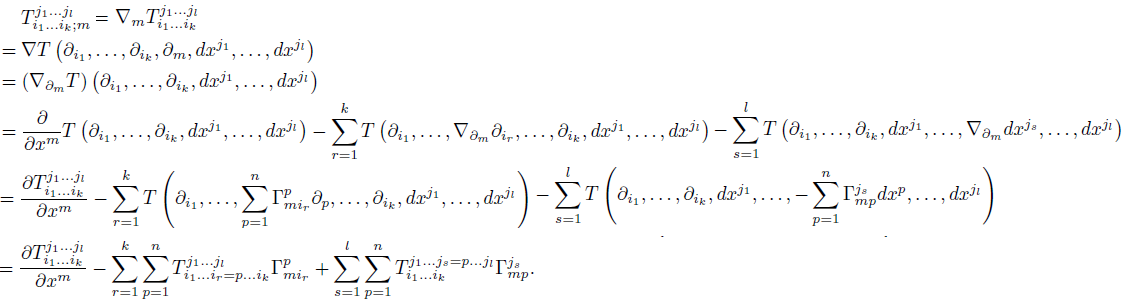
\includegraphics[scale=.67]{deriv_total_christoffel}
		\end{center}

	\section{Quest\~ao de Lee 5.4, p. 87}
		\begin{flushright}
		\end{flushright}

		(a) Relembre que $V$ \'e paralelo se $\nabla V \equiv 0$. Sejam $p \in \mathbb{R}^n, V_p \in T_p \mathbb{R}^n$. Prove que $V_p$ tem extens\~ao \'unica a campo vetorial paralelo $V$ em $\mathbb{R}^n$.

		Fixamos $n = 3, p = (1,0,0), V_p = (0, a, b), \Gamma = 0$.

		$\nabla_{\alpha'} V = \cfrac{dV^1}{dt} \partial_x + \cfrac{dV^2}{dt} \partial_y + \cfrac{dV^3}{dt} \partial_z = 0 \Rightarrow V(t) = V_p$

		Em particular, $V = V_p$ nas curvas $\alpha_i(t) = p + t \cdot e_i, i \in \{ 1,2,3 \}$

		Portanto, a extens\~ao \'unica \'e $V \equiv V_p$.

		\vspace{3mm}

		(b) Sejam em $S^2$, coordenadas esf\'ericas $(\theta, \varphi)$. Seja $V = \partial_\varphi$. Ent\~ao $\nabla V(Z) = \nabla_Z V = f \nabla_{\partial_\theta}V + g\nabla_{\partial_\varphi}V$.

		Utilizamos gr.pdf 3.2 p\'agina 62:

		$\nabla_{\partial_\theta} \partial_\varphi = \Gamma_{12}^1 \partial_\theta + \Gamma_{12}^2 \partial_\varphi\,;\nabla_{\partial_\varphi} \partial_\varphi = \Gamma_{22}^1 \partial_\theta + \Gamma_{22}^2 \partial_\varphi$

		$\Gamma_{22}^1 = - \sin \varphi \cos \varphi, \Gamma_{12}^2 = \Gamma_{21}^2 = \cot \varphi$, o resto \'e zero. A cotangente estoura nos polos $\pm N$.

		$\nabla_{\partial_\theta} \partial_\varphi = \cot \varphi \cdot \partial_\varphi\,;\nabla_{\partial_\varphi} \partial_\varphi = - \sin \varphi \cos \varphi \cdot \partial_\theta$

		Conclua que $V$ \'e paralelo ao longo do equador $\varphi = \cfrac{\pi}{2}$ e ao longo de cada meridiano $\theta = \theta_0$.

		$\varphi = \cfrac{\pi}{2} \Rightarrow 0 = \nabla_{\partial_\theta} \partial_\varphi = \nabla_{\partial_\varphi} \partial_\varphi$

		$\theta = \theta_0 \Rightarrow \alpha(t) = (\theta(t), \varphi(t)) = (\theta_0, t) \Rightarrow \alpha'(t) = (0, 1)$

		$Y = V \circ \alpha$

		$V^1 = 0 \Rightarrow W^1 = \cfrac{DY}{dt} = \nabla_{\alpha'} (\partial_\varphi) = $
		$\cfrac{d\alpha^1}{dt} \Gamma_{12}^1 V^2 \partial_1 + \cfrac{d\alpha^2}{dt} \Gamma_{22}^1 V^2 \partial_1$
		$+ \cfrac{d\alpha^1}{dt} \Gamma_{12}^2 V^2 \partial_2 + \cfrac{d\alpha^2}{dt} \Gamma_{22}^2 V^2 \partial_2$

		$W_p^1 = - \cfrac{d\varphi}{dt} \sin \varphi \cos \varphi V^2 \partial_\theta + \cfrac{d\theta}{dt} \cot \varphi V^2 \partial_\varphi = - \sin t \cos t \partial_\theta$

		$W_p^1(f) = - \sin t \cos t \cfrac{\partial f}{\partial \theta} = 0$ sempre que $f$ independe de $\theta$. $V$ \'e paralelo ao longo das fun\c{c}\~oes constantes em rela\c{c}\~ao \`a longitude. Cada c\'irculo m\'aximo \'e o equador, por assim dizer, em alguma base $B$. Mais uma vez: esta teoria \'e local, n\~ao global. Localmente, ``aqui" tem latitude zero e longitude arbitr\'aria. O eixo de rota\c{c}\~ao da Terra deixa de ser o eixo $z$.

		\vspace{3mm}

		(c) Seja $p$ em $\theta = 0, \varphi = \cfrac{\pi}{2}$. Prove que $V_p$ n\~ao tem nenhuma extens\~ao paralela a nenhuma vizinhan\c{c}a de $p$.

		$p = (1,0,0) \in \mathbb{R}^3$. Seja $\alpha(1) = (\epsilon, \pi/2 + \epsilon) \Rightarrow \alpha(t) = (t, \pi/2 + t) \Rightarrow \alpha'(t) = (1, 1)$

		$V = \delta \partial_\theta + (1 + \delta) \partial_\varphi$. Queremos mostrar que $\nabla V \ne 0$. Primeiro perturbamos o ponto. Depois perturbamos o vetor tangente.

		$\nabla_{\partial_\theta + \partial_\varphi} \partial_\varphi = \cot \varphi \cdot \partial_\varphi - \sin \varphi \cos \varphi \cdot \partial_\theta = W^2$

		O \'unico jeito de $W^2 = 0$ \'e se $f =$ constante. Caso contr\'ario, $\varphi = \pi/2 + \epsilon \Rightarrow W^2 \ne 0$.

		O caso $\alpha(t) = (t, \pi/2)$ \'e desconsiderado por ser unidimensional. Abertos aqui t\^em dimens\~ao 2.

		$\nabla_{\alpha'} [t \partial_\theta + (1 + t) \partial_\varphi] = t \nabla_{\alpha'} \partial_\theta + (1 + t) W^2 = W^3$

		$\nabla_{\partial_\theta + \partial \varphi} \partial_\theta = [\cancel{\Gamma_{11}^1} \partial_1 + \cancel{\Gamma_{11}^2} \partial_2] + [\cancel{\Gamma_{21}^1} \partial_1 + \Gamma_{21}^2 \partial_2]$

		$W^3 = t \cot \varphi \cdot \partial_\varphi  + (1 + t) W^2 \ne 0$, simplesmente porque $t = \delta$ e $W^2 \ne 0$.

		\vspace{3mm}

		(d) Utilize a, c para provar que nenhuma vizinhan\c{c}a de $p$ \'e isom\'etrica a um aberto de $\mathbb{R}^2$.

		Em $\mathbb{R}^2$, o campo vetorial constante $V \equiv V_p$ \'e paralelo globalmente.

		Se houvesse isometria, em $S^2$ haveria um campo vetorial paralelo qualquer definido em um aberto qualquer de $S^2$.

		Mas isso \'e absurdo, porque em $S^2$, os campos paralelos s\~ao unidimensionais, definidos somente ao longo de curvas: o equador e os meridianos.

	\section{Quest\~ao de Manfredo 2.7}
		\begin{flushright}
		\end{flushright}

		Em $S^2$, seja $c$ um paralelo e $V_0$ um vetor tangente a $S^2$ em um ponto de $c$. Descreva geometricamente o transporte paralelo de $V_0$ ao longo de $c$ em $S^2$.

		Para tanto, considere o cone $C$ tangente a $S^2$ ao longo de $c$ e prove que \'e id\^entico ao transporte paralelo de $V_0$ ao longo de $c$ em $C$.

		\vspace{3mm}

		Coordenadas de $c$: $\alpha(t) = (\theta(t), \varphi(t)) = (t, \varphi_0) \Rightarrow \alpha'(t) = (1, 0)$.

		Seja $p = c(0) = (0, \varphi_0)$. Ent\~ao $p = (\sin \varphi_0, 0, \cos \varphi_0) \in \mathbb{R}^3\,; V_p = (a, b) \in T_pS^2$.

		Equa\c{c}\~oes diferenciais em $V$:

		$\cfrac{dV^1}{dt} + \cfrac{d\alpha^1}{dt} \Gamma_{11}^1 V^1  + \cfrac{d\alpha^1}{dt} \Gamma_{12}^1 V^2  + \cfrac{d\alpha^2}{dt} \Gamma_{21}^1 V^1  + \cfrac{d\alpha^2}{dt} \Gamma_{22}^1 V^2 = 0$

		$\cfrac{dV^2}{dt} + \cfrac{d\alpha^1}{dt} \Gamma_{11}^2 V^1  + \cfrac{d\alpha^1}{dt} \Gamma_{12}^2 V^2  + \cfrac{d\alpha^2}{dt} \Gamma_{21}^2 V^1  + \cfrac{d\alpha^2}{dt} \Gamma_{22}^2 V^2 = 0$

		In\'icio em: $V^1(0) = a, V^2(0) = b$.

		Substitu\'imos:

		$\cfrac{dV^1}{dt} = 0, V^1(0) = a \Rightarrow V^1(t) \equiv a$

		$\cfrac{dV^2}{dt} + \cot \varphi_0 \cdot V^2 = 0 \Rightarrow y' + ky = 0 \Rightarrow y(t) = C \exp(-kt) \Rightarrow y(0) = C \therefore V^2(t) = b \exp (-\cot \varphi_0 t)$

		Para $\varphi_0 \ne \cfrac{\pi}{2} + k\pi$, podemos completar a base com $\partial_\theta = (\cos \varphi_0, 0, -\sin \varphi_0 \cos t)\,; \partial_\varphi = (0, \cos \varphi_0, -\sin \varphi_0 \sin t)$.

		Lembrando que a base come\c{c}a com $\alpha(t) = (\sin \varphi_0 \cos t, \sin \varphi_0 \sin t, \cos \varphi_0)$.

		O plano tangente ``f\'isico" \'e $\{ v(t) = \alpha + \lambda \partial_\theta + \mu \partial_\varphi \,; \lambda, \mu \in \mathbb{R} \}$.

		O cone s\'o piora as coisas. $z = \cos \varphi_0\,; x^2 + y^2 = (A z)^2 \Rightarrow A = \tan \varphi_0$.

		Exemplo: $\varphi_0 = \cfrac{\pi}{4} \Rightarrow V(t) = a \cdot \partial_\theta + b \cdot e^{-t} \partial_\varphi$. Trata-se de um vetor tangente em $T_pS^2$ com m\'odulo decrescendo exponencialmente com o tempo. Podemos completar a base com $\partial_\varphi = \bigg(0, \cfrac{\sqrt 2}{2}, -\cfrac{\sqrt 2}{2} \cdot \sin t\bigg)$, que d\'a $V(t)$ depois de multiplicado por $b \cdot e^{-t}$.

		O cone \'e $z = \cfrac{\sqrt 2}{2}\,; x^2 + y^2 = z^2$. $\alpha(t) = \bigg(\cfrac{\sqrt 2}{2}\cdot \cos t, \cfrac{\sqrt 2}{2}\cdot \sin t, \cfrac{\sqrt 2}{2}\bigg)$. Interessante que $V(2\pi) = e^{-2\pi} V_p$, quando $a = 0$.

	\section{Quest\~ao de Manfredo 2.5, p. 64}
		\begin{flushright}
		\end{flushright}

		No espa\c{c}o euclideano, o transporte paralelo de 1 vetor entre 2 pontos n\~ao depende da curva que liga esses 2 pontos.

		D\^e exemplo de que isso n\~ao \'e verdade em uma variedade de Riemann qualquer.

		\vspace{3mm}

		A pen\'ultima quest\~ao mostra em $\mathbb{R}^n$ o transporte paralelo constante globalmente $V \equiv V_p$.

		A \'ultima mostra tamb\'em que em $S^2$ o transporte paralelo $V(t)$ depende do par\^ametro $t$ da curva $\alpha$.

	\section{Quest\~ao 9.31 de variedades\_diferenciaveis.pdf}
		\begin{flushright}
		\end{flushright}

		Todo 2-tensor \'e soma de sim\'etrico e alternado. Isso n\~ao \'e v\'alido para tensores de grau superior.

		\vspace{3mm}

		Primeiro: $\forall T^m \in \mathcal{T}^2(M), \exists\, T_{sim}, T_{alt}\,; T^m = T_{sim} + T_{alt}$

		Demo: Fa\c{c}a $T_{sim} = \text{Sim }T^m$ e $T_{alt} = \text{Alt }T^m$.$\,\,\blacksquare$

		\vspace{3mm}

		Exemplos:

		$du \otimes dv = \text{Sim}(du \otimes dv) + \text{Alt}(du \otimes dv)$

		$du \otimes dv \otimes dw \ne \text{Sim}(du \otimes dv \otimes dw) + \text{Alt}(du \otimes dv \otimes dw)$

		\begin{align*}
		T &= \sum_{i_1, \cdots, i_k = 1}^n T_{i_1, \cdots, i_k} du^{i_1}\otimes \cdots \otimes du^{i_k} \\
		\text{Sim } T &= \sum_{i_1, \cdots, i_k = 1}^n \cfrac{1}{k!} \sum_{\sigma \in S_k} T_{\sigma(i_1), \cdots, \sigma(i_k)} du^{i_1}\otimes \cdots \otimes du^{i_k} \\
		\text{Alt } T &= \sum_{i_1, \cdots, i_k = 1}^n \cfrac{1}{k!} \sum_{\sigma \in S_k} (\text{sgn } \sigma) T_{\sigma(i_1), \cdots, \sigma(i_k)} du^{i_1}\otimes \cdots \otimes du^{i_k}
		\end{align*}

		$T$ \'e sim\'etrico se $T(v_1, \cdots, v_i, \cdots, v_j, \cdots, v_k) = T(v_1, \cdots, v_j, \cdots, v_i, \cdots, v_k)$.

		$T$ \'e alternado se $T(v_1, \cdots, v_i, \cdots, v_j, \cdots, v_k) = - T(v_1, \cdots, v_j, \cdots, v_i, \cdots, v_k)$.

		\vspace{3mm}

		Segundo: $\exists\, T^m \in \mathcal{T}^3(M), \forall\, X_{sim}, \forall\, Y_{alt}\,; T^m \ne X_{sim} + Y_{alt}$

		$6$ Sim $(du \otimes dv \otimes dw) = du \otimes dv \otimes dw + dw \otimes du \otimes dv + dv \otimes dw \otimes du + dv \otimes du \otimes dw + du \otimes dw \otimes dv + dw \otimes dv \otimes du$

		$6$ Alt $(du \otimes dv \otimes dw) = du \otimes dv \otimes dw + dw \otimes du \otimes dv + dv \otimes dw \otimes du - dv \otimes du \otimes dw - du \otimes dw \otimes dv - dw \otimes dv \otimes du$

		$($Sim $+$ Alt$)(du \otimes dv \otimes dw) = \cfrac{du \otimes dv \otimes dw + dw \otimes du \otimes dv + dv \otimes dw \otimes du}{3}$

		Vamos provar que \'e imposs\'ivel decompor. Seja a decomposi\c{c}\~ao absurda

		$du \otimes dv \otimes dw(v_1, v_2, v_3) = v_1^1 v_2^1 v_3^1 = X_{sim}(v_1, v_2, v_3) + Y_{alt}(v_1, v_2, v_3)$.

		\begin{align*}
		X_{sim} &= \sum_{i_1 = 1}^3 \sum_{i_2 = 1}^3 \sum_{i_3 = 1}^3 X_{i_1, i_2, i_3} du^{i_1} \otimes du^{i_2} \otimes du^{i_3} \\
		Y_{alt} &= \sum_{i_1 = 1}^3 \sum_{i_2 = 1}^3 \sum_{i_3 = 1}^3 Y_{i_1, i_2, i_3} du^{i_1} \otimes du^{i_2} \otimes du^{i_3} \\
		X + Y &= 1 du^1 \otimes du^2 \otimes du^3 = 1(123)\text{, por abuso de nota\c{c}\~ao}
		\end{align*}

		$X(v_1, v_2, v_3) = X(v_1, v_3, v_2) = X(v_3, v_1, v_2) = X(v_3, v_2, v_1) = X(v_2, v_3, v_1) = X(v_2, v_1, v_3)$

		$Y(v_1, v_2, v_3) = - Y(v_1, v_3, v_2) = Y(v_3, v_1, v_2) = - Y(v_3, v_2, v_1) = Y(v_2, v_3, v_1) = - Y(v_2, v_1, v_3)$

		\vspace{3mm}

		$X = A(123) + A(132) + A(312) + A(321) + A(231) + A(213)$
		$ + B(112) + B(121) + B(211) + C(113) + C(131) + C(311)$

		$ + D(122) + D(212) + D(221) + E(133) + E(313) + E(331)$
		$ + F(223) + F(232) + F(322) + G(233) + G(323) + G(332)$

		$ + H(111) + J(222) + K(333)$

		\vspace{3mm}

		$Y = A'(123) - A'(132) + A'(312) - A'(321) + A'(231) - A'(213)$
		$ + B'(112) - B'(121) + B'(211) + C'(113) - C'(131) + C'(311)$

		$ + D'(122) - D'(212) + D'(221) + E'(133) - E'(313) + E'(331)$
		$ + F'(223) - F'(232) + F'(322) + G'(233) - G'(323) + G'(332)$

		$ + H'(111) + J'(222) + K'(333)$

		\vspace{3mm}

		$A + A' = 1$

		$A - A' = 0 \Rightarrow A = A' = \cfrac{1}{2}$

		Imposs\'ivel cancelar $(A + A')(312)$ Q.E.A. $\,\,\blacksquare$

		\section{Grupos de Lie}
		\begin{flushright}
		\end{flushright}

		\subsection{5-10: Constantes de estrutura}
		\begin{flushright}
		\end{flushright}

		Em uma \'algebra de Lie $\mathcal{G}$, seja a base $(X_1, \cdots, X_n)$. Defina as constantes de estrutura $[X_i, X_j] = \sum_k c_{ij}^k X_k$. Compute Christoffel em termos de $c_{ij}^k, g_{ij}$.

		\vspace{3mm}

		Seja $n = 2$.

		$X_1 = X_1^1 \partial_1 + X_1^2 \partial_2 \Rightarrow \langle X_1, X_1 \rangle = 1^2$

		$X_2 = X_2^1 \partial_1 + X_2^2 \partial_2 \Rightarrow \langle X_2, X_2 \rangle = 1^2 \Rightarrow \langle X_1, X_2 \rangle = 0$

		$X_i = a \partial_1 + b \partial_2$

		$X_j = c \partial_1 + d \partial_2$

		$X_k = e \partial_1 + f \partial_2$

		$[X_i, X_j] = \underbrace{(a \partial_1 c - c \partial_1 a + b \partial_2 c - d \partial_2 a)}_\lambda \partial_1 + \underbrace{(a \partial_1 d - c \partial_1 b + b \partial_2 d - d \partial_2 b)}_\mu \partial_2$

		$[X_i, X_i] = 0 \Rightarrow c_{ii}^k = 0$

		\vspace{3mm}

		Sejam $i = 1, j = 2$.

		$[X_i, X_j] = c_{12}^1 X_i + c_{12}^2 X_j = \nabla_{X_i} X_j - \nabla_{X_j} X_i = \lambda\partial_1 + \mu\partial_2 = c_{12}^1X_i + c_{12}^2X_j = c_{12}^1a \partial_1 + c_{12}^1b \partial_2 + c_{12}^2c \partial_1 + c_{12}^2d \partial_2$

		$[X_j, X_i] = c_{21}^1 X_i + c_{21}^2 X_j = \nabla_{X_j} X_i - \nabla_{X_i} X_j = - c_{12}^1 X_i - c_{12}^2 X_j$

		$\lambda = c_{12}^1a + c_{12}^2c$

		$\mu = c_{12}^1b + c_{12}^2d$

		$c_{12}^1 = \cfrac{\lambda d - \mu c}{a d - b c} = \cfrac{(X_1^1 \partial_1 X_2^1 - X_2^1 \partial_1 X_1^1 + X_1^2 \partial_2 X_2^1 - X_2^2 \partial_2 X_1^1) X_2^2 - (X_1^1 \partial_1 X_2^2 - X_2^1 \partial_1 X_1^2 + X_1^2 \partial_2 X_2^2 - X_2^2 \partial_2 X_1^2) X_2^1}{X_1^1 X_2^2 - X_1^2 X_2^1}$

		$c_{12}^2 = \cfrac{- \lambda b + \mu a}{a d - b c} = \cfrac{- (X_1^1 \partial_1 X_2^1 - X_2^1 \partial_1 X_1^1 + X_1^2 \partial_2 X_2^1 - X_2^2 \partial_2 X_1^1) X_1^2 + (X_1^1 \partial_1 X_2^2 - X_2^1 \partial_1 X_1^2 + X_1^2 \partial_2 X_2^2 - X_2^2 \partial_2 X_1^2) X_1^1}{X_1^1 X_2^2 - X_1^2 X_2^1}$

		\vspace{3mm}

		Sejam $i,j,k \in \{1,2\}$.

		$\nabla_{X_i} X_j = \nabla_{a \partial_1 + b \partial_2} (c \partial_1 + d \partial_2)  = c \nabla_{a \partial_1 + b \partial_2} (\partial_1) + d \nabla_{a \partial_1 + b \partial_2} (\partial_2) = ac \nabla_{ \partial_1} \partial_1 + ad \nabla_{\partial_1} \partial_2 + bc \nabla_{\partial_2} \partial_1 + bd \nabla_{ \partial_2} \partial_2$

		$\nabla_{(a,b)} (c,d) = ac(\Gamma_{11}^1 \partial_1 + \Gamma_{11}^2 \partial_2) + ad(\Gamma_{12}^1 \partial_1 + \Gamma_{12}^2 \partial_2) + bc(\Gamma_{21}^1 \partial_1 + \Gamma_{21}^2 \partial_2) + bd(\Gamma_{22}^1 \partial_1 + \Gamma_{22}^2 \partial_2) = \alpha \partial_1 + \beta \partial_2$

		$\langle \nabla_{X_i} X_j, X_k \rangle = \cfrac{1}{2} \cdot (X_i\langle X_j,X_k\rangle + X_j\langle X_i,X_k\rangle - X_k\langle X_i,X_j\rangle - \langle X_i, [X_j,X_k]\rangle - \langle X_j, [X_i,X_k]\rangle + \langle X_k, [X_i,X_j]\rangle)$

		$= \cfrac{1}{2} \cdot (X_i\langle X_j,X_k\rangle + X_j\langle X_i,X_k\rangle - X_k\langle X_i,X_j\rangle - \langle X_i, c_{12}^1X_j + c_{12}^2X_k\rangle - \langle X_j, c_{12}^1X_i + c_{12}^2X_k\rangle + \langle X_k, c_{12}^1X_i + c_{12}^2X_j\rangle)$

		$= \cfrac{1}{2} \cdot [X_i (P) + X_j (Q) - X_k(R) + (c_{12}^1 - c_{12}^2)Q - 2 c_{12}^1 R] = \alpha e g_{11} + (\alpha f + \beta e) g_{12} + \beta f g_{22}$

		$= ac S\Gamma_{11}^1  + ad S\Gamma_{12}^1 + bc S\Gamma_{21}^1 + bd S\Gamma_{22}^1 + acT\Gamma_{11}^2 + adT \Gamma_{12}^2 + bcT\Gamma_{21}^2 + bdT \Gamma_{22}^2$

		$= \langle (acS, adS, bcS, bdS, acT, adT, bcT, bdT) , \Gamma \rangle_8$

		$= S (\sum \Delta_{ij} \Gamma_{ij}^1) + T (\sum \Delta_{ij} \Gamma_{ij}^2) = \langle [g] \cdot [X_k], [\Delta]_{1 \times 4} \cdot [\Gamma^1 | \Gamma^2]_{4 \times 2} \rangle_2$

		$= e (\sum \Delta_{ij} \Gamma_{ij}^1) g_{11} + f (\sum \Delta_{ij} \Gamma_{ij}^1) g_{12} + e (\sum \Delta_{ij} \Gamma_{ij}^2) g_{12} + f (\sum \Delta_{ij} \Gamma_{ij}^2) g_{22}$

		$P = c e g_{11} + (c f + d e) g_{12} + d f g_{22}$

		$Q = a e g_{11} + (a f + b e) g_{12} + b f g_{22}$

		$R = ac g_{11} + (ad + bc) g_{12} + bd g_{22}$

		$S = e g_{11} + f g_{12}$

		$T = e g_{12} + f g_{22} \Rightarrow (S, T) = [g] \cdot [X_k]$

		$\alpha = ac\Gamma_{11}^1  + ad\Gamma_{12}^1 + bc\Gamma_{21}^1 + bd\Gamma_{22}^1$

		$\beta = ac\Gamma_{11}^2  + ad\Gamma_{12}^2  + bc\Gamma_{21}^2  + bd\Gamma_{22}^2$

		$\Delta = [X_i] \cdot [X_j]^T$

		$X_i (P) + X_j (Q) - X_k(R) + (c_{12}^1 - c_{12}^2)Q - 2 c_{12}^1 R = 2e (\sum \Delta_{ij} \Gamma_{ij}^1) g_{11} + 2f (\sum \Delta_{ij} \Gamma_{ij}^1) g_{12} + 2e (\sum \Delta_{ij} \Gamma_{ij}^2) g_{12} + 2f (\sum \Delta_{ij} \Gamma_{ij}^2) g_{22}$

		S\~ao 8 linhas. 6 linearmente independentes. 121 = 211. 122 = 212. A partir daqui, $X_1 = (a,b), X_2 = (c,d)$.

		$P_1^1 = a^2 g_{11} + 2ab g_{12} + b^2 g_{22}$

		$P_1^2 = a c g_{11} + (a d + b c) g_{12} + b d g_{22}$

		$P_2^2 = c^2 g_{11} + 2cd g_{12} + d^2 g_{22}$

		$Q_1^2 = (2 a^2 - ac) g_{11} + (4ab - ad - bc) g_{12} + (2b^2 - bd) g_{22}$

		$R_1^2 = (2ac - a^2) g_{11} + (2bc + 2ad - 2ab) g_{12} + (2bd - b^2) g_{22}$

		$R_2^1 = (c^2 - 2ac) g_{11} + (2cd - 2ad - 2bc) g_{12} + (d^2 - 2bd) g_{22}$

		$A_{32} = a(ad+bc) g_{11} + b(ad+bc) g_{12}$

		$A_{42} = c(ad+bc) g_{11} + d(ad+bc) g_{12}$

		$A_{35} = a(ad+bc) g_{12} + b(ad+bc) g_{22}$

		$A_{45} = c(ad+bc) g_{12} + d(ad+bc) g_{22}$

		Se as duas linhas abaixo n\~ao forem verdadeiras, o sistema \'e imposs\'ivel. Falta considerar $n \ge 3$.

		$c \partial_1 P_1^1 + d \partial_2 P_1^1 - c_{12}^1 R_1^2 - c_{12}^2 P_1^1 = a \partial_1 P_1^1 + b \partial_2 P_1^1 - c_{12}^1 P_1^2 - c_{12}^2 P_1^2$

		$a \partial_1 P_2^2 + b\partial_2 P_2^2 - c_{12}^1 P_1^2 - c_{12}^2 P_1^2 = c \partial_1 P_2^2 + d \partial_2 P_2^2 + c_{12}^1 R_2^1 - c_{12}^2 P_2^2$

		$\therefore 2 A \Gamma = B - c_{12}^1 V - c_{12}^2 W \Rightarrow \Gamma = \cfrac{1}{2}\cdot A^{-1} (B - c_{12}^1 V - c_{12}^2 W)$

		\vspace{3mm}

		$2 \left[ \begin{matrix} a^3 g_{11} + a^2b g_{12} & 2a^2b g_{11} + 2ab^2 g_{12} & ab^2 g_{11} + b^3 g_{12} & a^3 g_{12} + a^2b g_{22} & 2a^2b g_{12} + 2ab^2 g_{22} & ab^2 g_{12} + b^3 g_{22} \\ a^2 c g_{11} + a^2 d g_{12} & 2abc g_{11} + 2abd g_{12} & b^2c g_{11} + b^2d g_{12} & a^2c g_{12} + a^2d g_{22} & 2abc g_{12} + 2abd g_{22} & b^2c g_{12} + b^2d g_{22} \\ a^2c g_{11} + abc g_{12} & A_{32} & abd g_{11} + b^2d g_{12} & a^2c g_{12} + abc g_{22} & A_{35} & abd g_{12} + b^2d g_{22} \\ ac^2 g_{11} + acd g_{12} & A_{42} & bcd g_{11} + bd^2 g_{12} & ac^2 g_{12} + acd g_{22} & A_{45} & bcd g_{12} + bd^2 g_{22} \\ ac^2 g_{11} + bc^2 g_{12} & 2acd g_{11} + 2bcd g_{12}  & ad^2 g_{11} + bd^2 g_{12} & ac^2 g_{12} + bc^2 g_{22} & 2acd g_{12} + 2bcd g_{22} & ad^2 g_{12} + bd^2 g_{22} \\ c^3 g_{11} + c^2d g_{12} & 2c^2d g_{11} + 2cd^2 g_{12} & cd^2 g_{11} + d^3 g_{12} & c^3 g_{12} + c^2d g_{22} & 2c^2d g_{12} + 2cd^2 g_{22} & cd^2 g_{12} + d^3 g_{22} \end{matrix} \right]\cdot \left[ \begin{matrix} \Gamma_{11}^1 \\ \Gamma_{12}^1 \\ \Gamma_{22}^1 \\ \Gamma_{11}^2 \\ \Gamma_{12}^2 \\ \Gamma_{22}^2 \end{matrix} \right]$

		$= \left[ \begin{matrix} a \partial_1 P_1^1 + b \partial_2 P_1^1 \\ a \partial_1 Q_1^2 + b \partial_2 Q_1^2 \\ c \partial_1 P_1^1 + d \partial_2 P_1^1  \\ a \partial_1 P_2^2 + b\partial_2 P_2^2 \\ -c \partial_1 R_2^1 - d\partial_2 R_2^1  \\ c \partial_1 P_2^2 + d\partial_2 P_2^2 \end{matrix} \right] - c_{12}^1 \left[ \begin{matrix} P_1^1 \\ Q_1^2 \\ R_1^2  \\ P_1^2  \\ R_2^1 \\ P_2^2 \end{matrix} \right] - c_{12}^2 \left[ \begin{matrix}  P_1^1 \\ P_1^2 \\ P_1^1 \\ P_1^2 \\ P_1^2 \\ P_2^2 \end{matrix} \right]$

		\vspace{120mm}

		Era s\'o o produto interno. Agora \'e tensor.

		Era s\'o tangente. Agora \'e tensor.

		Era s\'o derivar. Agora \'e tensor.

		Era s\'o matriz linha e coluna. Agora \'e tensor covariante e contravariante.

		Era s\'o matriz c\'ubica. Agora \'e tensor trilinear.

		Era s\'o uma matriz computacional int$[3][3][3][3][3]$. Agora \'e quase um tensor de $\mathbb{Z}^3$.

		Era s\'o a faixa de Moebius. Raio e \^angulo. Agora tem fibrado pra tudo quanto \'e lado. kkk

\end{document}
